\documentclass[a4paper,12pt]{report}
\usepackage{times}
\usepackage{graphicx}
\usepackage[a4paper,
bindingoffset=0.2in,
left=1in,
right=.5in,
top=.7in,
bottom=.5in,
footskip=.25in]{geometry}
\begin{document}
	\begin{center}
		\textbf{NETACODE -A SOFTWARE COMPANY VISITING REPORT}\\
		\begin{flushleft}
			The report is visiting a software company for \textbf{Course tittle:Information System Design with industrial attachment Sessional} Course and \textbf{Course Code:CSE 3210} in Computer Science and Engineering.\\
		\end{flushleft}
				by\\	
			Mst.Habiba Hena Sumi(200101070)\\Most.Jannat-Ul-Ferdoush(200101068)\\Md.Talath Un Nabi(200101076)\\Ferdous Tahsin(200101079)\\
			
			\begin{figure}[h]
				\centering
				\includegraphics[width=0.4\linewidth]{"images (1)"}
				\label{fig:images-1}
			\end{figure}
		
		\vspace{1 cm}
			Submited To:\\
			Teacher name:Ananna Hoque Shathi\\
			Department of Computer Science and Engineering(CSE)\\
			Bangladesh Army University of Science and Technology(BAUST)\\
			
		\end{center}
	
	\begin{flushright}
		\vspace{3 cm}
		...............................................\\
		signature of the teacher
	\end{flushright}
\newpage
\tableofcontents
\listoffigures
\listoftables
\newpage

\chapter{Systems Concepts and the Information Systems Environment}
\section{INTRODUCTION}
 System analysis and design is a process that many companies use to evaluate particular business situations and develop ways to improve them through more optimal methods.\\
 
\section {Characteristic of System:}
\textbf{Organization}
Their organization has a branch in Dinajpur district. Netacode is a multinational software company. Main office in Dhaka in Bangladesh. Their organizations are certainly very beautiful. 4 storied building and their number of rooms is 7.\\

\textbf{Interaction}
It is defined by the manner in which the components operate with each other.For example, in an organization,purchasing department must interact with production department and payroll with personnel department.\\

\textbf{Interdependence}
Interdependence means how the components of a system depend on one another. For proper functioning, the components are coordinated and linked together according to a specified plan. \\

\textbf{Integration}
Integration is concerned with how a system components are connected together. It means that the parts of the system work together within the system even if each part performs a unique function.\\

\textbf{Central Objective}
The objective of system must be central. It may be real or stated. It is not uncommon for an organization to state an objective and operate to achieve another.\\
\begin{figure}[h]
	\centering
	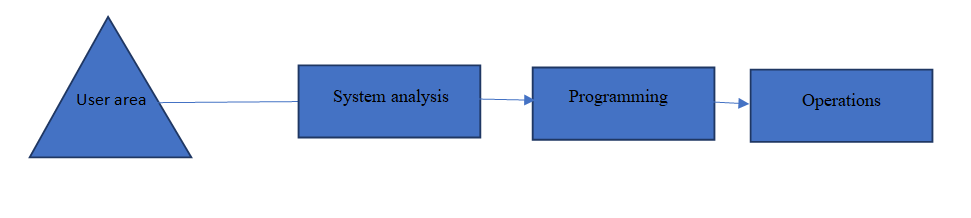
\includegraphics[width=0.7\linewidth]{1}
	\caption{Task Interdependence in a Computer – Based Subsystem }
	\label{fig:1}
\end{figure}
\section{Elements of System}
\textbf{Outputs and Inputs}
\begin{itemize}
	\item 	The main aim of a system is to produce an output which is useful for its user.
	\item 	Inputs are the information that enters into the system for processing.
	\item 	Output is the outcome of processing.
\end{itemize}
\textbf{Processor(s)}
\begin{itemize}
	\item 	The processor is the element of a system that involves the actual transformation of input into output.
	\item 	It is the operational component of a system. Processors may modify the input either totally or partially, depending on the output specification.
\end{itemize}
\textbf{control}
\begin{itemize}
	\item The control element guides the system.
	\item	It is the decision–making subsystem that controls the pattern of activities governing input, processing, and output.
\end{itemize}
\textbf{Feedback}
\begin{itemize}
	\item Feedback provides the control in a dynamic system.
	\item	Positive feedback is routine in nature that encourages the performance of the system.
	\item	Negative feedback is informational in nature that provides the controller with information for action.
\end{itemize}
\textbf{Environment}
\begin{itemize}
	\item	The environment is the “supersystem” within which an organization operates.
	\item	It is the source of external elements that strike on the system.
\end{itemize}
\textbf{Boundaries and Interface}
\begin{itemize}
	\item	A system should be defined by its boundaries. Boundaries are the limits that identify its components, processes, and interrelationship when it interfaces with another system.
	\item	Each system has boundaries that determine its sphere of influence and control.
\end{itemize}
\begin{figure}[h]
	\centering
	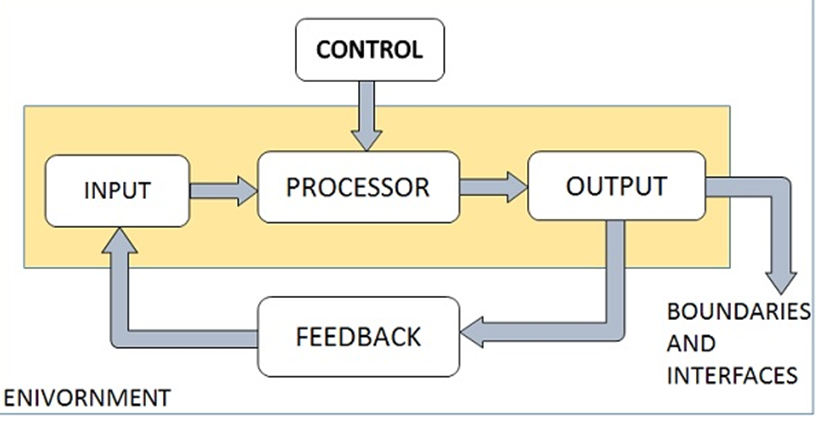
\includegraphics[width=0.7\linewidth]{2}
	\label{fig:2}
\end{figure}
\section{Types of Systems}
The systems can be divided into the following types 
\textbf{Physical or Abstract Systems}
\begin{itemize}
	\item	Physical systems are tangible entities. We can touch and feel them.
	\item	Physical System may be static or dynamic in nature. For example, desks and chairs are the physical parts of computer center which are static. A programmed computer is a dynamic system in which programs, data, and applications can change according to the user's needs.
	\item	Abstract systems are non-physical entities or conceptual that may be formulas, representation or model of a real system.
\end{itemize}
\textbf{Open or Closed Systems}
\begin{itemize}
	\item	An open system must interact with its environment. It receives inputs from and delivers outputs to the outside of the system. For example, an information system which must adapt to the changing environmental conditions.
	\item	A closed system does not interact with its environment. It is isolated from environmental influences. A completely closed system is rare in reality.
\end{itemize}
\begin{figure}[h]
	\centering
	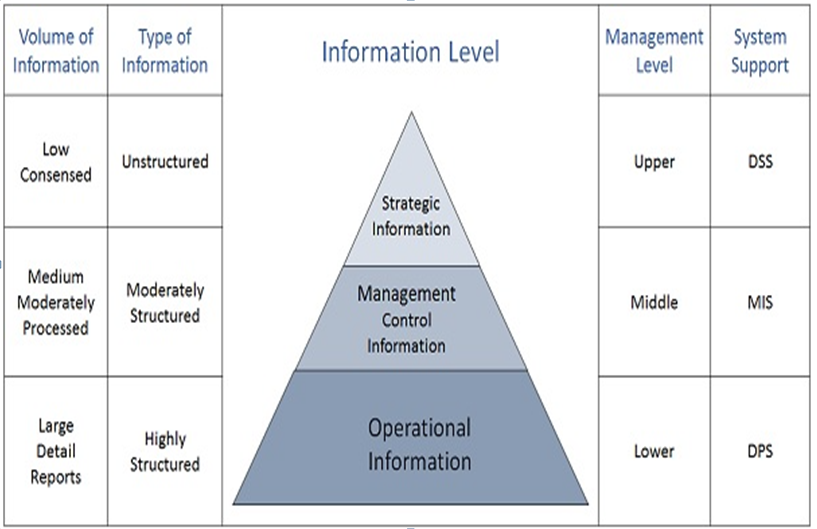
\includegraphics[width=0.7\linewidth]{3}
	\caption{Categories of information related to managerial levels and the decision managers make.}
	\label{fig:3}
\end{figure}
\newpage
\textbf{Goals}\\
To provide trouble-free, customer-focused, reliable, and affordable web hosting services. WE simply want
to continue to operate a profitable web hosting company that makes customers happy. \\Since the
beginning, we have backed our rock solid hosting solutions and top-notch infrastructure with the best
customer service and technical support. A common feeling about the technology field is it's all about
machines, yes, It does take machines but, Host Pair also knows it takes good people to run a well-oiled
machine. Yes, a successful business needs to be committed to client solutions, innovation, creativity, and
a warm, caring attitude to all of our customers' business needs. We don't just provide 24x7 support. We
really do listen and care.













\newpage
\chapter{The System Development Life Cycle }
\section{Introduction:}
The system development life cycle is a conceptual model used for project management that describes the stages involved in an information system development project,from an initial feasibility study through maintainence of the completed application. To understand system development,we need to recognize that a candidate system has a life cycle. The stages are shown below:
\begin{enumerate}
	\item Recognititon of need / initial investigation
	\item	Feasibility Study
	\item	Analysis
	\item Design
	\item	Implementation
	\item	Post-implementation and maintenance   
	\end{enumerate}
\begin{figure}[h]
	\centering
	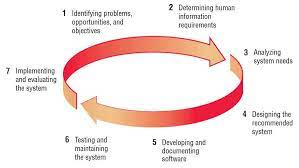
\includegraphics[width=0.7\linewidth]{fig-1;chap-2}
	\caption{System development life cycle}
	\label{fig:fig-1chap-2}
\end{figure}
\section{Recognition of Need: }
One must know what the problems are before it can be solved. The basis for a candidate system is recognition of a need for improving an information system or a procedure. For example, a supervisor wants to investigate the system flow in purchasing.When we have completed our visit at netacode ,we discuss the recognition needs of their clients and how they collect and process the requirements to complete their project  successfully. They told us they have arranged meetings with their clients many times to understand and collect the requirements. They provide them forms and other documents to understand what is the actual need of their clients.If the problem is serious enough , management may want to have an analyst look at it. Such assignment  implies a commitment. At this stage only a rough estimation of the development cost of the project may be reached.If the problem is serious enough , management may want to have an analyst look at it. Such assignment  implies a commitment. At this stage only a rough estimation of the development cost of the project may be reached.
\section{Feasibility Study}
Depending on the initial investigation the survey expanded to a more detailed feasibility study. It is the test of a system proposal according to its workability. It focuses on three major questions:
\begin{enumerate}
	\item 	What are the users demonstrable needs and how does a candidate system meet them?
	\item	What resources are available for a given candidate system? Is the problem worth solving?
	\item	What are likely impacts of the candidate system on the organization? How does it fit within the organization MIS plan?
	\end{enumerate}
Each of these questions must be answered carefully. They revolved around the investigation and evaluation of the problem,identification and description of the candidate system,specification of performance and the cost of each system and final selection of the best system.\\ \\

The objective of the feasibility study is not to solve the problem but to acquire a sense of its scope. During the study the problem definition is crystalized and aspects of the problem to be included in the system are determined.\\ \\

The proposal summarizes what is known and what is going to be done. It is consist of the following:
\begin{enumerate}
	\item \textbf{Statement of the problem :} A carefully worded statement of the problem led to analysis.
	
	\item \textbf{	Summary of the findings and recommendations :} A list of the major findings and recommendations of the study. It is the idea for the user who requires quick access to the results of the analysis of the system under study. Conclusions are started followed by a list of the recommendations and a justification for them.
	
	\item \textbf{ Details of the findings :} an outline of the methods are procedures undertaken by the existing system,followed by coverage of the objectives and procedures of the candidate system. Included are also discussions of output reports, file structures, and cost and benefits of the candidate system.
	
	\item \textbf{	Recommendation and conclusions :} Specific recommendations regarding the candidate system, including personnel assignments, costs, project schedules and target dates.
\end{enumerate}
\section{Analysis:}
 It is the detailed study of the various operations performed by a system and their relationships within and outside of the system. A key question is : what must be done to solve the problem?\\ 
 
 When we visited the organization we discussed the analysis system. They first analys if they are able to complete it or not and then they discuss further processes that are steps they should take to make the project successful. Training, experience and common sense are required for collection of the information needed to do the analysis.
 \\ \\
 Once the analysis is completed, the analyst has a firm understanding what is to be done. The next step is to decide how the problem must be solved. Thus in system design, we move from the logical to physical aspects of the life cycle of a project.\\
 \section{Design:}
 The most creative and challenging phase of a system life cycle of a project is system design. The term design describes a final system and the process by which it is developed. It refers to the technical specifications that will be applied in implementing the project. The question is here: How should the problem be solved?\\
 
\begin{figure}[h]
	\centering
	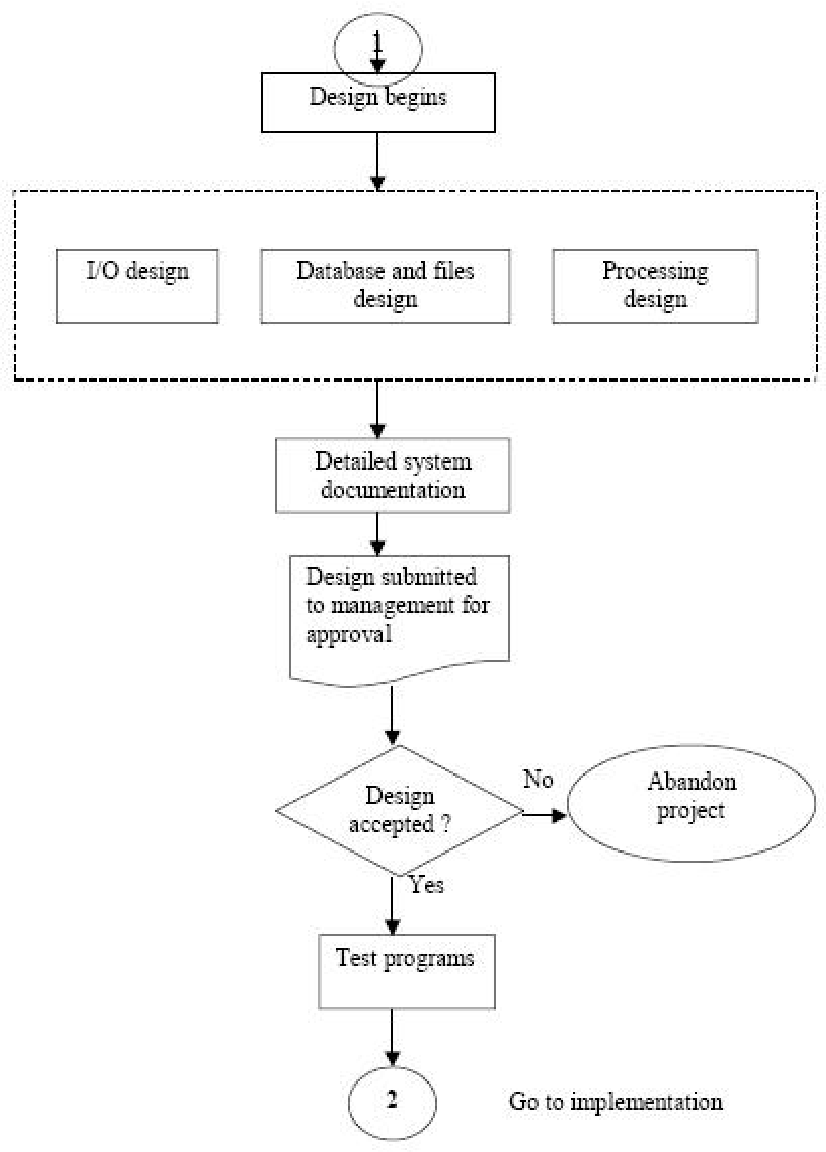
\includegraphics[width=0.7\linewidth]{fig-2;chap-2}
	\caption{design of a system}
	\label{fig:fig-2chap-2}
\end{figure}
The first step is to determine how the output is to be produced and in what form. Samples of the output are also presented. Second, input data and master files  are designed to meet the requirements of the proposed output. Finally details related to justification of the project and an estimate of the impact of the candidate system on the user and the organization  are documented and evaluated by management as a step toward implementation.
\\ \\
In netacode they first create a virtual design of the project by adobe illustrator or figma.then they present it to their clients to justify if it has been according to their requirements or not.\\
In some firms, separate groups of programmers do the programming , whereas other firms employ analyst programmers who do analysis.
\section{Implementation:}
The implementation sector is less creative than system design. It is primarily concerned with user training, site preparation and file conversion. Depending on the nature of the system, extensive user training may be required. Conversion usually takes place at about the same time the user is being trained or later.\\

In netacode they told us they used  react js as frontend development and node js for backend development. They also use nuxt js and next js for development. They used php but now they have shifted to javascript. \\

Once the program becomes available,test data is read into the computer and  processed against the file(s) provided for testing. If successful, the program(s) is then run with live data. Otherwise  a diagnostic procedure is used to locate and correct errors in the program. In most conversions a parallel run is conducted where the new system runs simultaneously with the old system. 
\section{Post termination and Maintenance : }
After the installation phase is completed and the user stuff is adjusted to the changes created by the candidate system, evaluation and  maintenance begin. Like any system, there is an aging process that requires periodic maintenance of hardware and software. If the new information is inconsistent with the design specifications, the changes have to be made. The importance of maintenance is to continue to bring the new system to standards.\\ 

The policy of Netacode is to serve their clients with the project they have created according to the requirements. but they don't share the source code of any project and if their updates are available, they do it take charges. This is their strategy of post implementation and maintenance of any project.



\end{document}
